\section{Global Optimization}

Optimization is a field of applied mathematics that deals with finding the best
set of parameters to optimize an objective function. A problem with $N$
variables $\{n_0, \dots, n_{N-1}\}$ in range $n_i \in \{0, \dots, k-1\}$ will
have a search space with $k^N$ possible solutions. Each solution can be
evaluated by applying the objective function to it, to obtain the solutions
\emph{fitness}. The fitness is a measure of how good the solution is and is used
to assist the selection of candidate solutions for evaluation.

In general, the possible solution can be thought of as a space that has two or
more dimensions, directly related to the number of variables in the solution
in addition to one axis for calculated fitness. If a problem contains a single
variable, its solution space might look like \autoref{fig:fitnesslandscape}
where the X-axis is the value of the single variable, while the Y-axis is the
fitness of this solution. Problems with more variables will have more axis. The
optimization algorithms can be thought of as methods for exploring and finding
the highest or lowest point in of the fitness-axis.

As both $k$ and $N$ grow large, it becomes infeasible to search through and
evaluate the vast amount of permutations. In such cases, other techniques must
be employed. Finding an arbitrary local minimum is often straight forward using
classical \emph{local} optimization methods such as the Simple Hill Climbing
Algorithm. However, these methods cannot always be used to find a global minimum
\cite{russellnorvig}. A wide range of algorithms to search through a subset of
the solution space exists, each with different approaches and properties.
\autoref{fig:metaheuristics} shows a map of how different optimization
algorithms are related to each other. Most of these are described in detail in
\cite{russellnorvig}.

\begin{figure}[bth]
    \centering
    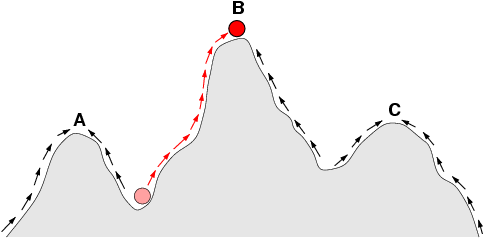
\includegraphics[width=0.8\textwidth]{figs/Fitness-landscape-cartoon.png}
    \caption{Sketch of a fitness landscape, borrowed from \cite{wikifitnesslandscape}}
    \label{fig:fitnesslandscape}
\end{figure}

On a high level, optimization algorithms can be divided into deterministic and
non-deterministic approaches. The deterministic approaches can be thought of as
a single path in solution space that starts at a defined but most likely
suboptimal solution and ends at the best solution, while the non-deterministic
approaches usually selects one or more paths by random such that each run might
have a different outcome. Deterministic algorithms will always find the same
solution, but if the search space is large enough, this might take extremely
long time do.  With the case of non-deterministic algorithms, they tend to have
an explorative behaviour \cite{poli2008field}; each computation of next state
includes some form of randomness. E.g. simulated annealing will do the same as
the hill climbing algorithm, but will have some chance of moving downhill, thus
it will be less prone to be stuck in a local minima. We will now provide a brief
overview of algorithms considered for use in this thesis.


\begin{description}
    \item[Regression] is described as a study of dependence between properties
        \cite{weisberg2005applied}. When set data set contains values from at
        least two properties, regression can be used to find one value as a
        function of the other. The simplest form of regression is the linear
        regression. A linear regression will try to find the linear function,
        $y=a_1x_1+a_2x_2+...+a_nx_n+b$, that minimizes the least square error.
        Common for implementation of linear regression solvers is to formulate
        the problem as a system of linear equations \cite{lay2011linear}, which
        can be solved by Gaussian elimination. More advanced forms for
        regressions can be used when the problem cannot be well mapped with a
        linear function, such as the Gauss-Newton algorithm
        \cite{myers1990classical}.

    \item[Simulated Annealing] is a technique that belongs to the field of
        stochastic optimization and metaheuristics, inspired by the process of
        annealing in metallurgy \cite{van1987simulated}. Initially, it starts in
        a random state $s$ and for each iteration it probabilistically decides
        between moving the system to a neighboring state $s'$ or staying in in
        state $s$. To avoid ending up in a local minima, the probability starts
        high, but decreases after time. Hence, simulated annealing quickly
        considers the most important parts of the state if configured adequately.

    \item[Evolutionary Algorithms] is a term that refers to computational
        methods inspired by the process and mechanisms of biological evolution
        \cite{fogel1997evolutionary}.  They differ from conventional algorithms
        by selecting the best-fit individuals in a population for reproduction
        and applying crossover and mutation to produce offspring. Only the best
        fit individuals go on to the next generation \cite{introtoga}.

\end{description}

\begin{figure}
    \centering
    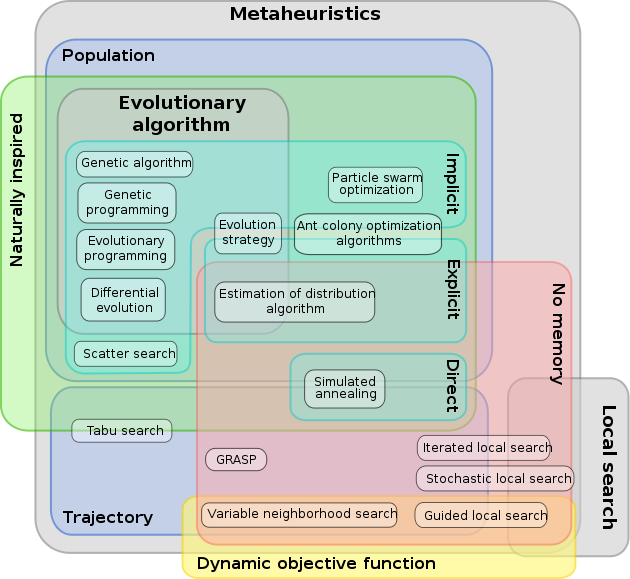
\includegraphics[width=0.8\textwidth]{figs/630px-Metaheuristics_classification.png}
    \caption{Different classifications of searching algorithms, borrowed from Johann "nojhan" Dréo and Caner Candan \cite{wikimetaheuristics}}
    \label{fig:metaheuristics}
\end{figure}

Global optimization problems is a well studied research area and there is a
wealth of different ways to solve them. It can be difficult to know in advance
which methods will provide the most fruitful results. Also, multiple approaches
can be combined in efforts to extract the best properties from several worlds,
or to get the speed of convergence up.

